% !TeX root = 00P2_cep_semantics.tex
\clearpage
\section*{Appendix B. Worked Examples}
\addcontentsline{toc}{section}{Appendix B. Worked Examples}

This appendix provides concrete examples illustrating how the categorical
structures in the paper (functors, fibrations, oplax adapters) manifest
in realistic CEP workflows.

% ------------------------------------------------------------
\subsection*{B.1 Normalization and Canonicalization}
% ------------------------------------------------------------

Consider an entity with the following unnormalized fields:

\begin{mdframed}
  \textbf{Name:} ``City of Springfield'' \\
  \textbf{Address:} ``123 Lincoln Ave'' \\
  \textbf{Country:} ``US'' \\
  \textbf{Date:} (none)
\end{mdframed}

Applying the normalization functor
\[
  \mathcal{F}_{normalize} : \mathbf{R}_{raw} \to \mathbf{R}_{canon},
\]
yields:

\begin{mdframed}
  \textbf{Name:} ``city of springfield'' \\
  \textbf{Address:} ``123 lincoln ave'' \\
  \textbf{Country:} ``US'' \\
  \textbf{Date:} ``1900-01-01''
\end{mdframed}

The canonicalization functor
\[
  \mathcal{C} : \mathbf{R}_{canon} \to \mathbf{C}
\]
produces the canonical string:
\[
  \mathcal{C}(R)
  =
  \texttt{city of springfield|123 lincoln ave|US|1900-01-01}.
\]

The hashing endofunctor $H$ computes the identifier:
\[
  \text{SNFEI}(R) = H(\mathcal{C}(R)).
\]

This example illustrates strict monoidality: components are concatenated
in a fixed order, independent of non-identity updates.

% ------------------------------------------------------------
\subsection*{B.2 Envelope Functor and Attestation Naturality}
% ------------------------------------------------------------

Let $P$ be the canonical payload from Example B.1.

\[
  \mathcal{E}(P)
  = \text{Envelope with schema version and revision metadata},
\]
\[
  \mathcal{E}'(P)
  = \text{Envelope additionally carrying a digital attestation}.
\]

The natural transformation $\alpha : \mathcal{E} \Rightarrow \mathcal{E}'$
assigns
\[
  \alpha_P : \mathcal{E}(P) \to \mathcal{E}'(P),
\]
representing the application of attestation.

If $f : P \to P'$ is a valid record evolution, naturality ensures the
square

\[
  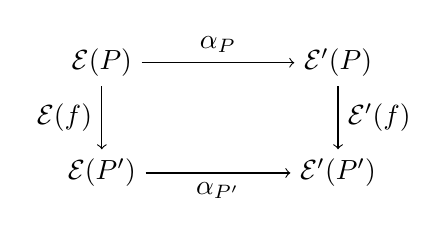
\begin{tikzpicture}[baseline=(current bounding box.center)]
    \node (EP)   at (0,0)     {$\mathcal{E}(P)$};
    \node (EPP)  at (3,0)     {$\mathcal{E}'(P)$};
    \node (EPp)  at (0,-1.4)  {$\mathcal{E}(P')$};
    \node (EPPp) at (3,-1.4)  {$\mathcal{E}'(P')$};
    \draw[->] (EP)   -- node[above] {$\alpha_P$}   (EPP);
    \draw[->] (EPp)  -- node[below] {$\alpha_{P'}$} (EPPp);
    \draw[->] (EP)   -- node[left]  {$\mathcal{E}(f)$} (EPp);
    \draw[->] (EPP)  -- node[right] {$\mathcal{E}'(f)$} (EPPp);
  \end{tikzpicture}
\]
commutes.
This expresses provenance consistency: attestation interacts
correctly with record evolution.

% ------------------------------------------------------------
\subsection*{B.3 Jurisdictional Adapters as Oplax Functors}
% ------------------------------------------------------------

Consider a local schema $\mathbf{J_{local}}$:

\begin{mdframed}
  \textbf{name}, \textbf{state}, \textbf{address}, \textbf{source-system}
\end{mdframed}

and a global CEP vocabulary $\mathbf{J_{global}}$:

\begin{mdframed}
  \textbf{legalName}, \textbf{jurisdictionIso}, \textbf{location.address},\\
  \textbf{entityTypeUri}, \textbf{status}
\end{mdframed}

An adapter $\mathcal{A}$ maps:
\[
  \mathcal{A}(\texttt{name}) = \texttt{legalName}, \qquad
  \mathcal{A}(\texttt{state}) = \texttt{jurisdictionIso},
\]
\[
  \mathcal{A}(\texttt{address}) = \texttt{location.address},
\]
while \texttt{source-system} may map to optional metadata.

Optionality induces oplaxity:
\[
  \mathcal{A}(x) \otimes \mathcal{A}(y)
  \to
  \mathcal{A}(x \otimes y),
\]
which need not be invertible.
This models structure weakening in cross-jurisdiction transformations.

% ------------------------------------------------------------
\subsection*{B.4 Context Tags and Fiber Reindexing}
% ------------------------------------------------------------

Let $R$ be an entity record with SNFEI $s$.

The fiber $\mathbf{CT}_R$ contains allowable context tags such as:

\begin{mdframed}
  \texttt{analysis.cluster.membership: "cluster-17"} \\
  \texttt{quality.issue.incomplete\_address: true}
\end{mdframed}

If the record evolves via
\[
  f : R \to R',
\]
then the fibration provides a reindexing functor
\[
  f^\ast : \mathbf{CT}_{R'} \to \mathbf{CT}_R
\]
that keeps tags aligned with the record's evolution
without altering the underlying identifier $s$.
